The oil price data is shown in Figure~\ref{fig:oil}, which includes the monthly prices and the 12 month moving average.
\begin{figure}[H]
\centering
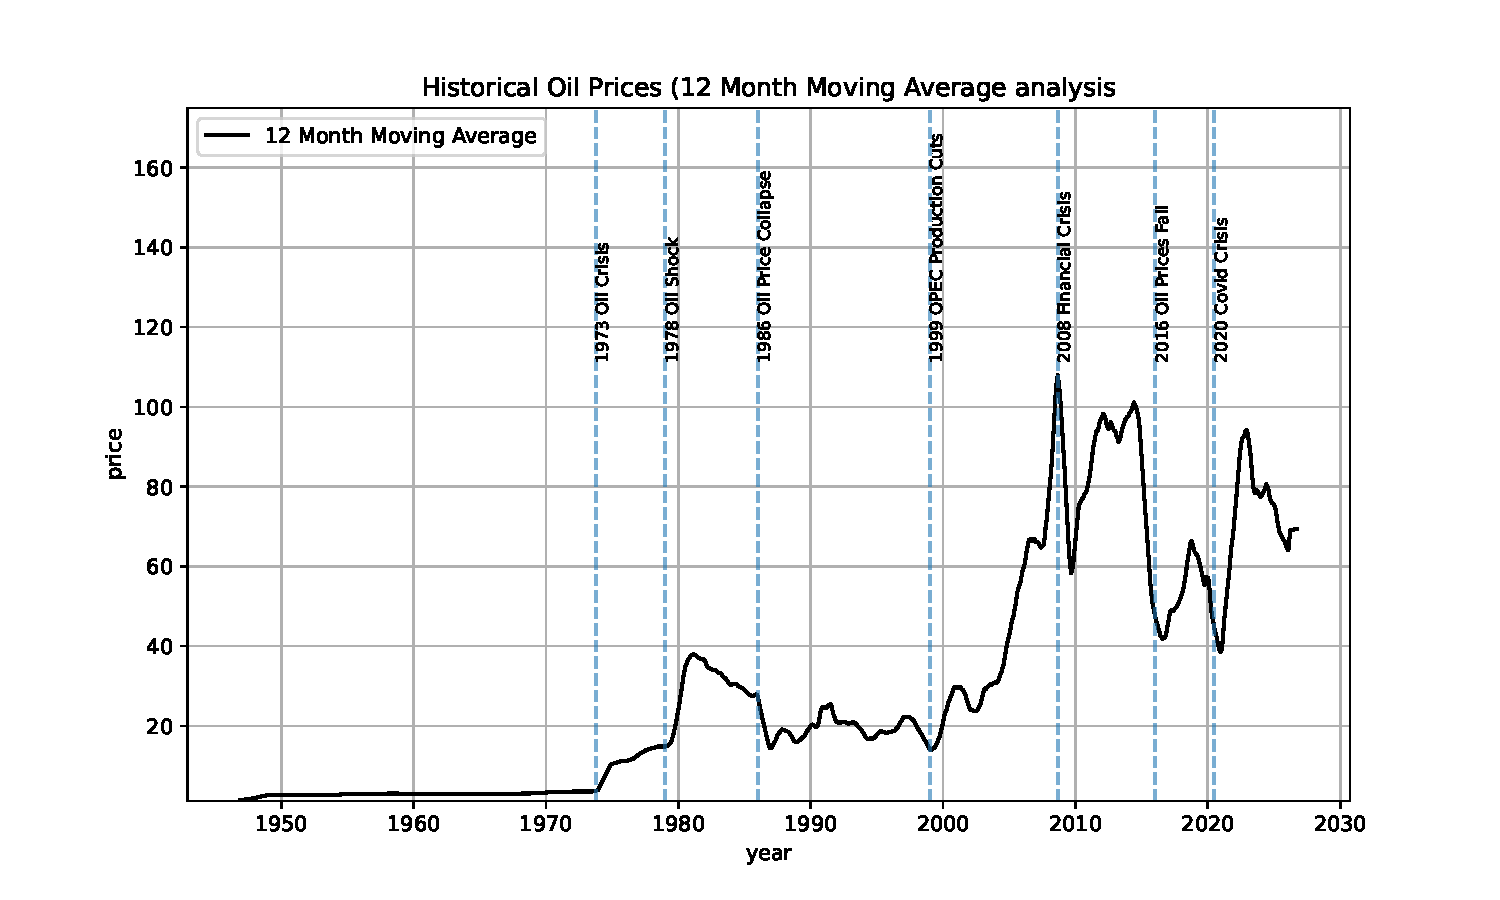
\includegraphics[width=0.9\textwidth]{oil_prices_plot.pdf}
\caption{Historical crude oil prices with a 12 month moving average and major economic events.}
\label{fig:oil}
\end{figure}
The results show clear patterns in the oil price data. We can see how the moving average made the peaks relatively smooth in order to better understand the peaks and troughs of oil prices. We can see sharp changes in price behavior and that they are connected to major global events.
